\chapter{Preliminary Study}

\section{Automatic Speech Recognition}

Automatic Speech Recognition (ASR) is the process of converting spoken language into text and has undergone significant evolution, progressing from traditional statistical pipelines to modern end-to-end neural architectures~\cite{graves2006ctc, chan2015las}. Its applications span a wide range of domains, including voice assistants, captioning, transcription, and accessibility technologies. Recent research has increasingly focused on enhancing robustness, supporting low-resource languages, and leveraging large-scale pretraining to improve generalization and reduce reliance on labeled data~\cite{baevski2020wav2vec2, radford2022whisper}.

\begin{figure}[h!]
    \centering
    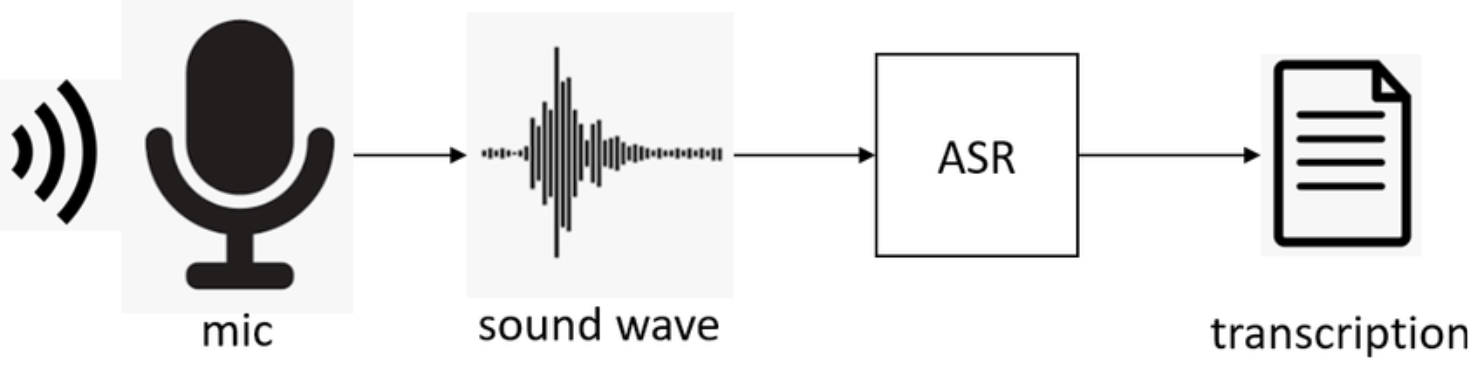
\includegraphics[width=0.9\textwidth]{img/pdz/09-asr-pipeline.png}
    \caption{ASR pipeline \cite{asr_pipeline_rg}}
    \label{fig:ASR_Pipeline}
\end{figure}

ASR is the task of converting an acoustic signal into a sequence of words. Formally, the goal of an ASR system is to determine the most probable word sequence $\hat{W}$ given an input acoustic observation $X$

\begin{equation*}
    \hat{W} = \arg\max_{W} P(W|X)
\end{equation*}

Using Bayes' theorem, this can be rewritten as

\begin{equation*}
    \hat{W} = \arg\max_{W} P(X|W)P(W)
\end{equation*}

where:
\begin{itemize}
    \item $P(X|W)$ is the \textbf{acoustic model}, representing the probability of observing the audio features given a word sequence;
    \item $P(W)$ is the \textbf{language model}, representing the prior probability of a word sequence in the target language;
    \item $\hat{W}$ is the final predicted transcription.
\end{itemize}

The decoder combines both models to search for the optimal word sequence.


The earliest generation of ASR systems was based on Gaussian Mixture Models (GMMs) combined with Hidden Markov Models (HMMs), which provided temporal alignment and probabilistic modeling of speech signals~\cite{hinton2012dnn, rabiner1989hmm}. These systems relied on n-gram language models and lexicons to capture linguistic structure. Around 2010–2015, the hybrid Deep Neural Network–HMM (DNN–HMM) approach emerged, where deep neural networks replaced GMMs to improve acoustic modeling~\cite{hinton2012dnn}. This hybrid paradigm dominated production ASR systems for several years, supported by widely used toolkits such as Kaldi~\cite{povey2011kaldi} and benchmark datasets like Switchboard and WSJ~\cite{switchboard1992, wsj1993}, until end-to-end models began demonstrating superior performance.

End-to-end ASR methods simplify traditional pipelines by directly mapping audio signals to text with a single neural model, allowing joint optimization of components. Three major paradigms have shaped this shift. Connectionist Temporal Classification (CTC) enables training without frame-level alignment by marginalizing over possible alignments, making it effective for character or phoneme-based outputs~\cite{graves2006ctc}. Attention-based encoder–decoder models, exemplified by Listen, Attend and Spell (LAS), rely on an encoder to produce representations and an attention mechanism to guide token-level predictions, effectively modeling dependencies between outputs~\cite{chan2015las}. Transducer models, such as the Recurrent Neural Network Transducer (RNN-T) and Transformer Transducer, combine alignment and prediction into a unified probabilistic framework that supports streaming and low-latency applications~\cite{graves2012rnnt, he2019transformertransducer}. Each paradigm has its own trade-offs: CTC models are simple but constrained by conditional independence assumptions, attention-based models excel in accuracy but are less suitable for streaming, while transducer models balance accuracy and real-time usability.

End-to-End ASR using Connectionist Temporal Classification (CTC) models the probability of a label sequence $Y$ by summing over all possible alignments $\pi$ that collapse to $Y$

\begin{equation*}
    P(Y|X) = \sum_{\pi \in \mathcal{B}^{-1}(Y)} P(\pi|X)
\end{equation*}

where $\mathcal{B}$ is the mapping that removes blanks and repeated labels from the alignment path.


The introduction of transformer architectures has further advanced ASR by enabling global context modeling through attention mechanisms. Conformer, a convolution-augmented Transformer, improves upon the pure transformer design by integrating convolutional modules that capture local acoustic patterns while preserving global attention, achieving state-of-the-art performance on standard benchmarks such as LibriSpeech~\cite{gulati2020conformer, panayotov2015librispeech}. These innovations have established transformers and conformers as the backbone of modern ASR systems.

In attention-based ASR models, the system generates the output transcription autoregressively, producing one token at a time conditioned on previous outputs and the encoded acoustic features. The probability of generating a transcription sequence $Y$ given the input speech features $X$ is formulated as

\begin{equation*}
    P(Y|X) = \prod_{t=1}^{T} P(y_t \mid y_{1:t-1}, X)
\end{equation*}

where:
\begin{itemize}
    \item $X$ is the input acoustic feature sequence extracted from the speech signal;
    \item $Y = (y_1, y_2, \dots, y_T)$ is the output sequence of tokens (e.g., characters, subwords, or words);
    \item $y_t$ is the token predicted at timestep $t$;
    \item $y_{1:t-1}$ denotes all previously generated tokens before timestep $t$;
    \item $T$ is the length of the output sequence;
    \item $P(y_t \mid y_{1:t-1}, X)$ is the conditional probability of generating token $y_t$ given the input features and prior predictions.
\end{itemize}

The decoder uses an attention mechanism to dynamically focus on relevant parts of the encoded speech representation at each timestep, enabling the model to learn soft alignments between acoustic frames and output tokens without explicit alignment labels.

Another major milestone is the rise of self-supervised learning and large-scale pretraining. Models such as wav2vec 2.0 learn powerful audio representations from unlabeled data using contrastive objectives and can be fine-tuned with limited labeled samples to achieve competitive Word Error Rates (WER)~\cite{baevski2020wav2vec2}. Large-scale efforts, including Whisper, demonstrate that scaling both data and model size improves robustness, generalization, and zero-shot transfer across languages and domains~\cite{radford2022whisper}. This trend highlights the growing importance of pretraining as a foundation for ASR development.

Datasets and benchmarks play a central role in evaluating ASR progress. LibriSpeech has become the primary benchmark for reporting performance~\cite{panayotov2015librispeech}, while datasets such as Switchboard~\cite{switchboard1992}, TED-LIUM~\cite{rousseau2012tedlium}, and Mozilla’s Common Voice provide additional testbeds across different domains and languages~\cite{ardila2020commonvoice}. Evaluation typically relies on Word Error Rate (WER) and Character Error Rate (CER), with WER remaining the most widely used metric for system comparison.

It measures the difference between the reference transcription and the hypothesis transcription produced by the system. WER is computed as

\begin{equation*}
    \text{WER} = \frac{S + D + I}{N}
\end{equation*}

where:
\begin{itemize}
    \item $S$ is the number of word substitutions;
    \item $D$ is the number of word deletions;
    \item $I$ is the number of word insertions;
    \item $N$ is the total number of words in the reference transcript.
\end{itemize}

A lower WER indicates better recognition performance, with $\text{WER} = 0$ representing a perfect transcription.

Despite advances, practical deployment of ASR introduces further challenges. Many systems still integrate external language models or employ shallow fusion during decoding to improve accuracy~\cite{gulati2020conformer}. Streaming requirements necessitate architectures tailored for low-latency inference, such as transducer models or streaming variants of attention mechanisms~\cite{he2019transformertransducer}. On-device ASR applications also demand model compression, quantization, and lightweight designs to meet computational and memory constraints~\cite{han2016deepcompression}.

Robustness, fairness, and safety remain open challenges in the field. ASR systems continue to struggle with noise, accents, microphone variability, and domain shifts~\cite{radford2022whisper}. Although large-scale pretraining and data augmentation mitigate some issues, performance disparities persist for underrepresented languages and accents~\cite{ardila2020commonvoice}. Furthermore, large ASR models can generate hallucinated transcriptions that appear plausible but are incorrect, necessitating confidence estimation and caution in safety-critical applications.

Emerging directions in ASR research include the development of multilingual and code-switching systems~\cite{radford2022whisper}, efficient streaming attention mechanisms for real-time transcription~\cite{he2019transformertransducer}, privacy-preserving and on-device solutions~\cite{han2016deepcompression}, and the integration of diarization and alignment for richer transcription outputs. These efforts align with the broader trend toward building general-purpose, reliable, and accessible speech recognition technologies.

ASR has advanced from early GMM–HMM systems to end-to-end neural architectures that leverage transformers, conformers, and self-supervised pretraining. While remarkable improvements have been achieved in accuracy and efficiency, challenges in robustness, fairness, and real-time deployment remain pressing. Future progress will likely depend on scaling laws, architectural innovations, and greater diversity in datasets and evaluation methodologies, ensuring that ASR systems become more equitable, reliable, and widely applicable.


\section{Optical Character Recognition}

Optical Character Recognition (OCR) has long been regarded as a cornerstone technology in the field of document analysis, enabling the automatic extraction of textual information from scanned documents and images. Over the years, its evolution has been marked by significant advancements, beginning with simple rule-based and template-matching approaches and progressing toward sophisticated deep learning models. Today, OCR systems achieve near-human performance across multiple domains, making them an essential component in automation, digitization, and intelligent data processing \cite{smith2007tesseract, chen2021textrecognition}.

\begin{figure}[h!]
    \centering
    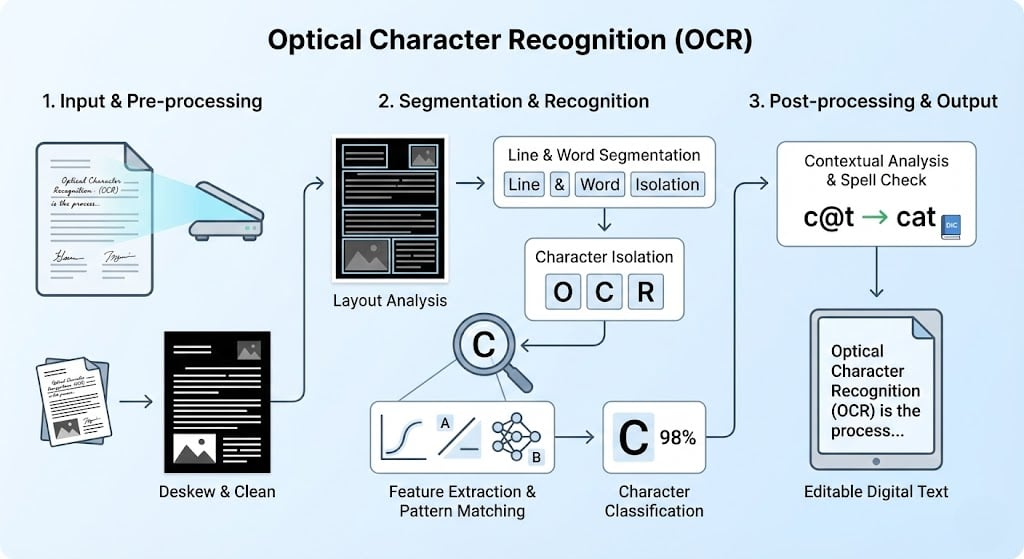
\includegraphics[width=0.9\textwidth]{img/pdz/10-ocr-pipeline.jpg}
    \caption{OCR pipeline.}
    \label{fig:OCR pipeline}
\end{figure}

The origins of OCR can be traced back to mechanical devices developed in the early 20th century, which were capable of recognizing characters in limited contexts. During the 1950s through the 1970s, template matching emerged as the dominant approach, though it was often constrained by sensitivity to font variations and document quality \cite{govindaraju1993handwritten}. By the 1970s, OCR technology saw commercial adoption in industries such as banking and postal services, where it was applied to automate check processing and mail sorting. Despite these advances, early commercial systems lacked robustness, often struggling with noise and inconsistencies in printed text \cite{mori1992historical}.

Conventional OCR pipelines were typically divided into sequential stages: segmentation, feature extraction, and classification. Early methods relied heavily on hand-crafted features such as zoning, projection profiles, and contour analysis, which were then processed using statistical classifiers, including Support Vector Machines (SVMs) and Hidden Markov Models (HMMs) \cite{casey1996survey}. While these approaches performed adequately for printed text, handwriting recognition posed greater challenges due to variability in writing styles, cursiveness, and the presence of ligatures. To address this, researchers explored techniques such as elastic matching and Dynamic Time Warping (DTW), which offered improved flexibility. Gradual integration of statistical modeling further enhanced performance, paving the way for more advanced approaches \cite{plamondon2000handwriting}.

The introduction of deep learning fundamentally transformed OCR research and practice. Convolutional Neural Networks (CNNs) proved especially effective for character recognition by learning spatial features directly from image data, eliminating the reliance on hand-crafted feature engineering \cite{lecun1998gradient}. Recurrent Neural Networks (RNNs) and their variants, particularly Long Short-Term Memory (LSTM) networks, enabled sequence modeling that supported recognition without explicit segmentation, addressing a key limitation of traditional systems \cite{graves2009novel}. Furthermore, the development of Connectionist Temporal Classification (CTC) provided alignment-free recognition of sequential text, significantly improving end-to-end performance \cite{graves2006ctc}. More recently, transformer-based architectures such as TrOCR have established the state of the art, offering robust recognition across a wide range of scripts and environmental conditions \cite{li2023trocr}.

With advances in deep learning, end-to-end models such as CRNN and Transformer-based architectures directly learn visual-to-text mappings from raw images \cite{shi2016crnn, baek2019deep, li2021trocr}. These models estimate the output text sequence by maximizing the conditional probability given the input image

\begin{equation*}
    \hat{Y} = \arg\max_{Y} P(Y|X)
\end{equation*}

where $X$ denotes the input image and $Y$ is the predicted text sequence.

Although OCR has significantly improved, challenges remain, including handwritten documents, low resolution images, domain-specific noise, multilingual text, and complex page layouts. These challenges motivate continued research toward more robust recognition models.

To evaluate OCR performance, character-level edit distance is widely used. The Character Error Rate (CER) is defined as

\begin{equation*}
    \text{CER} = \frac{S + D + I}{N}
\end{equation*}

where $S$, $D$, and $I$ are the number of substitutions, deletions, and insertions, respectively, and $N$ is the total number of reference characters. Word Error Rate (WER) applies the same formulation at the word level

\begin{equation*}
    \text{WER} = \frac{S + D + I}{N}
\end{equation*}

Lower CER and WER values indicate better recognition performance, thus motivating improvements in model architecture, data augmentation, and domain adaptation.

In addition to scanned documents, OCR research has increasingly focused on scene text recognition (STR), which addresses the challenges of extracting text embedded within natural images. Unlike structured documents, STR involves handling irregular backgrounds, distortions, and varying lighting conditions. To meet these challenges, recent methods have combined object detection frameworks such as Faster R-CNN and YOLO with recognition pipelines, thereby improving both localization and recognition accuracy. This integration has enabled OCR systems to achieve strong performance in real-world applications, where text often appears in unconstrained environments \cite{baek2019whatiswrong}.

The applications of OCR extend across diverse domains and industries, underscoring its versatility and impact. In the digital humanities, OCR plays a crucial role in large-scale digitization projects aimed at preserving and analyzing historical archives \cite{holley2009howgood}. Within the financial sector, it supports automated check verification and identity document processing, streamlining transactional workflows \cite{govindaraju1994handwritten}. In healthcare, OCR facilitates the digitization of medical prescriptions and patient records, enhancing accessibility and reducing manual entry errors \cite{zhou2022automatic}. Assistive technologies for visually impaired individuals also rely heavily on OCR, providing real-time access to printed information \cite{anagnostopoulos2006license}. Additionally, intelligent transportation systems employ OCR for automatic license plate recognition, contributing to improved traffic management and security \cite{du2013automatic}.

Despite remarkable progress, OCR continues to face several challenges that limit its universality. Multilingual recognition remains difficult, particularly for low-resource languages and scripts with limited annotated data \cite{smith2007tesseract}. Historical manuscripts and degraded documents introduce further complexity, as noise and damage hinder recognition accuracy \cite{chen2021textrecognition}. Handwriting variability remains an unresolved issue, with cursive and unconstrained writing styles posing significant obstacles \cite{plamondon2000handwriting}. Looking ahead, promising research directions include self-supervised learning approaches that reduce dependence on labeled data, multimodal OCR systems that integrate visual and linguistic cues, and few-shot learning methods designed to handle underrepresented languages effectively \cite{li2023trocr}.

OCR has undergone a profound transformation, evolving from rigid template-based recognition to flexible, data-driven deep learning and transformer-based systems. These advancements have enabled robust performance across a wide range of domains, from structured documents to complex natural scenes. As OCR continues to underpin automation, accessibility, and large-scale digitization efforts, ongoing research is likely to focus on improving its robustness, adaptability, and inclusivity. Future developments will ensure that OCR remains an indispensable technology in bridging the gap between visual and textual information.

\section{Transformer}
The Transformer model described in this section is based on the architecture proposed in \emph{Attention Is All You Need} by Vaswani et al.~\cite{vaswani2017attention}
The Transformer architecture, introduced by Vaswani et al. in 2017, revolutionized sequence modeling by relying entirely on self-attention mechanisms, dispensing with recurrent and convolutional structures. This design enabled efficient parallelization during training and excelled at capturing long-range dependencies, leading to state-of-the-art performance in natural language processing tasks such as machine translation, text generation, and language understanding.

\begin{figure}[h!]
    \centering
    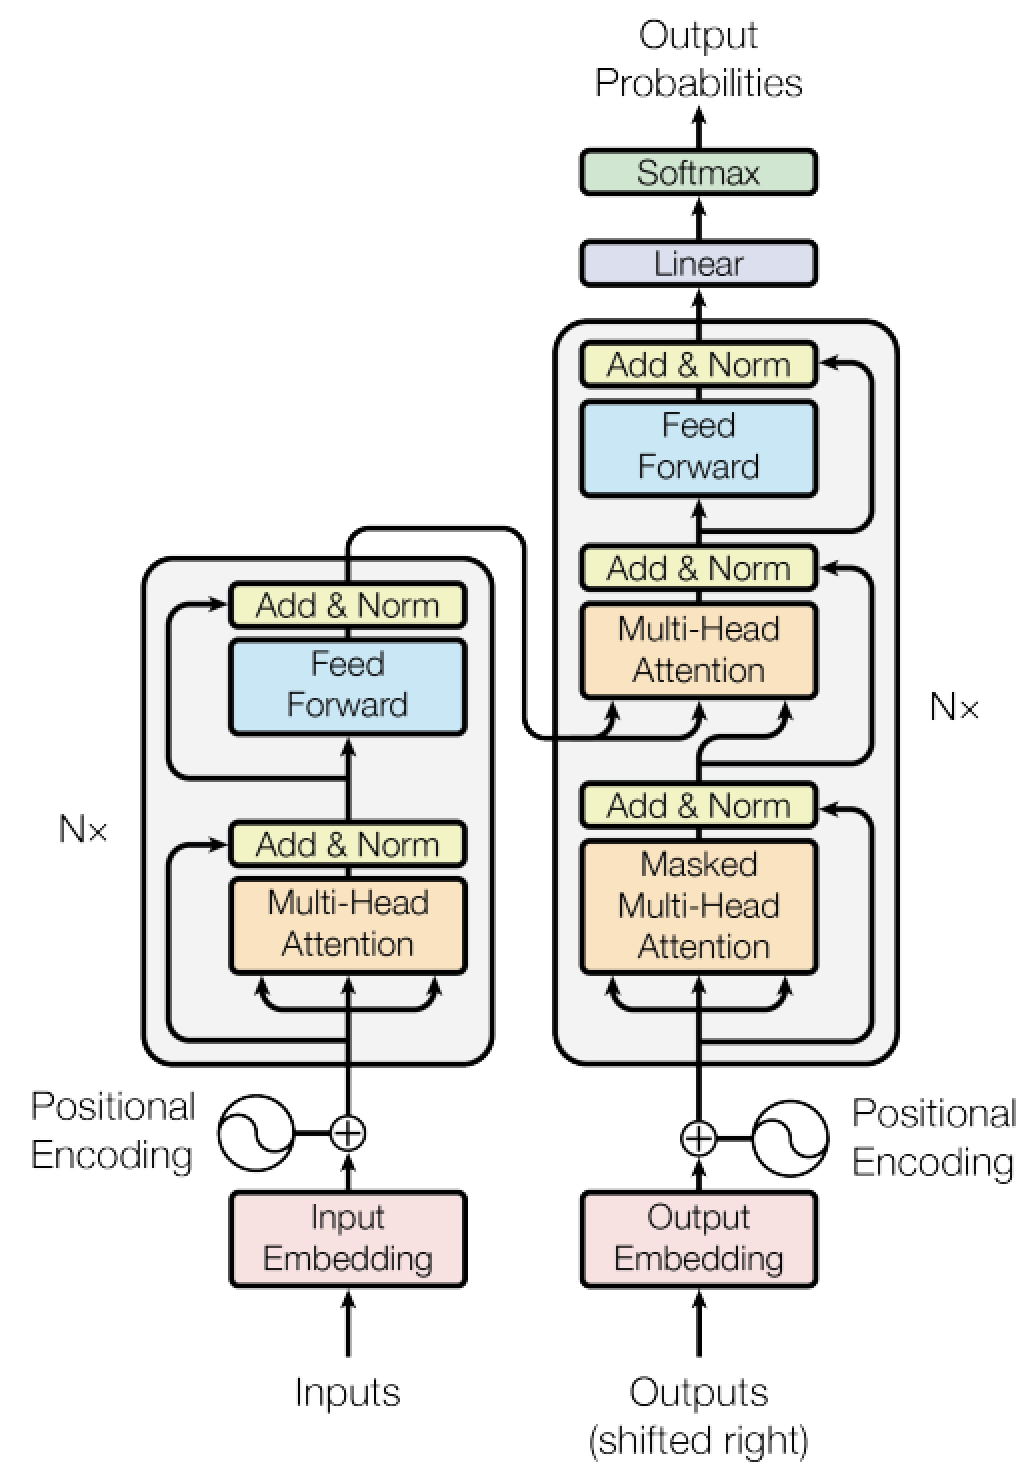
\includegraphics[width=0.5\textwidth]{img/pdz/06-transformers-architecture.png}
    \caption{The Transformer - model architecture.}
    \label{fig:Transformer architecture}
\end{figure}

A Transformer consists of an \textbf{Encoder} and a \textbf{Decoder}, each composed of $N$ identical layers ($N = 6$ in the original implementation).

Each Encoder layer contains two sub-layers:
\begin{enumerate}
    \item Multi-head self-attention.
    \item Position-wise fully connected feed-forward network.
\end{enumerate}
Each sub-layer is wrapped with a residual connection. Formally, the output of each sub-layer is
\[
\mathrm{LayerNorm}(x + \mathrm{Sublayer}(x)).
\]

Each Decoder layer contains three sub-layers:
\begin{enumerate}
    \item Masked multi-head self-attention, preventing each position from attending to future tokens.
    \item Multi-head attention over the Encoder outputs.
    \item Position-wise feed-forward network.
\end{enumerate}
As in the Encoder, residual connections and layer normalization are applied to each sub-layer.

Because the Transformer contains no recurrence or convolution, positional information must be injected explicitly. The model adds Positional Encodings to input embeddings at the bottoms of both the Encoder and Decoder stacks. The original Transformer uses sinusoidal encodings defined as
\[
\mathrm{PE}(pos, 2i) = \sin\left(\frac{pos}{10000^{2i / d_{\text{model}}}}\right),
\]
\[
\mathrm{PE}(pos, 2i+1) = \cos\left(\frac{pos}{10000^{2i / d_{\text{model}}}}\right),
\]
where $pos$ is the token position and $i$ is the dimension index. Each dimension corresponds to a sinusoid at a different frequency, enabling the model to encode both absolute and relative positional patterns.

Self-attention computes an output for each position by mapping a query vector to a set of key-value pairs.


Similarity between queries and keys is computed via the dot product $QK^{T}$, followed by a softmax to obtain attention weights. Because large values can destabilize gradients when the dimensionality $d_{K}$ is high, the dot products are scaled by $\sqrt{d_{K}}$
\[
\mathrm{Attention}(Q, K, V)
= \mathrm{softmax}\left( \frac{QK^{T}}{\sqrt{d_{K}}} \right) V.
\]

Instead of performing a single attention operation, the Transformer projects queries, keys, and values into $h$ subspaces using learned linear transformations. Attention is computed independently in each head
\[
\text{head}_{i} = \mathrm{Attention}(QW_i^{Q},\, KW_i^{K},\, VW_i^{V}).
\]
The outputs of all $h$ heads are concatenated and linearly transformed
\[
\mathrm{MultiHead}(Q,K,V) = 
\mathrm{Concat}(\text{head}_1, \ldots, \text{head}_h) W^{O}.
\]

This mechanism allows the model to capture multiple types of relationships simultaneously by attending to diverse representation subspaces.


\section{Multimodal Fusion and Cross-Attentional Models}

For specific data types and stages within retrieval pipelines, more specialized architectures are necessary. In the context of video, which inherently combine visual frames, audio signals, motion dynamics, and transcripts generated through automatic speech recognition, reliance on purely visual encoders such as CLIP fails to exploit the full range of available modalities. To address this limitation, the Multi-level Multi-modal Hybrid Fusion (M2HF) model has been proposed. This model integrates three complementary mechanisms. It first applies multi-stream feature extraction in order to capture representations from visual, audio, motion, and ASR-text channels. It then employs attentional fusion, where attention blocks are used to generate enriched cross-modal features, such as audio-guided visual representations, rather than relying on naive concatenation. Finally, it implements multi-level fusion strategies, combining modalities at both the feature level and the decision level, thereby producing richer and more informative retrieval signals~\cite{liu2022m2hf}.

Cross-attentional models constitute another important development, particularly in the reranking stage of retrieval pipelines. Unlike dual-encoder architectures, which encode queries and documents independently, cross-attentional models such as BERT-based cross-encoders compute deep, token-level interactions between queries and documents. This capacity allows them to capture fine-grained semantic distinctions, such as differentiating between “a slide explaining photosynthesis” and “a slide merely mentioning photosynthesis.” Their ability to model these nuanced relationships has consistently led to state-of-the-art performance in reranking tasks. However, these gains come at the cost of high computational complexity, which renders such models impractical for large-scale, first-stage retrieval~\cite{zhu2024reranking, yoo2021cooperative}. Instead, their most effective application lies in second-stage reranking, where they refine a smaller set of candidate results returned by a more efficient retrieval mechanism~\cite{pinecone2025rerankers}.

\begin{figure}[h!]
    \centering
    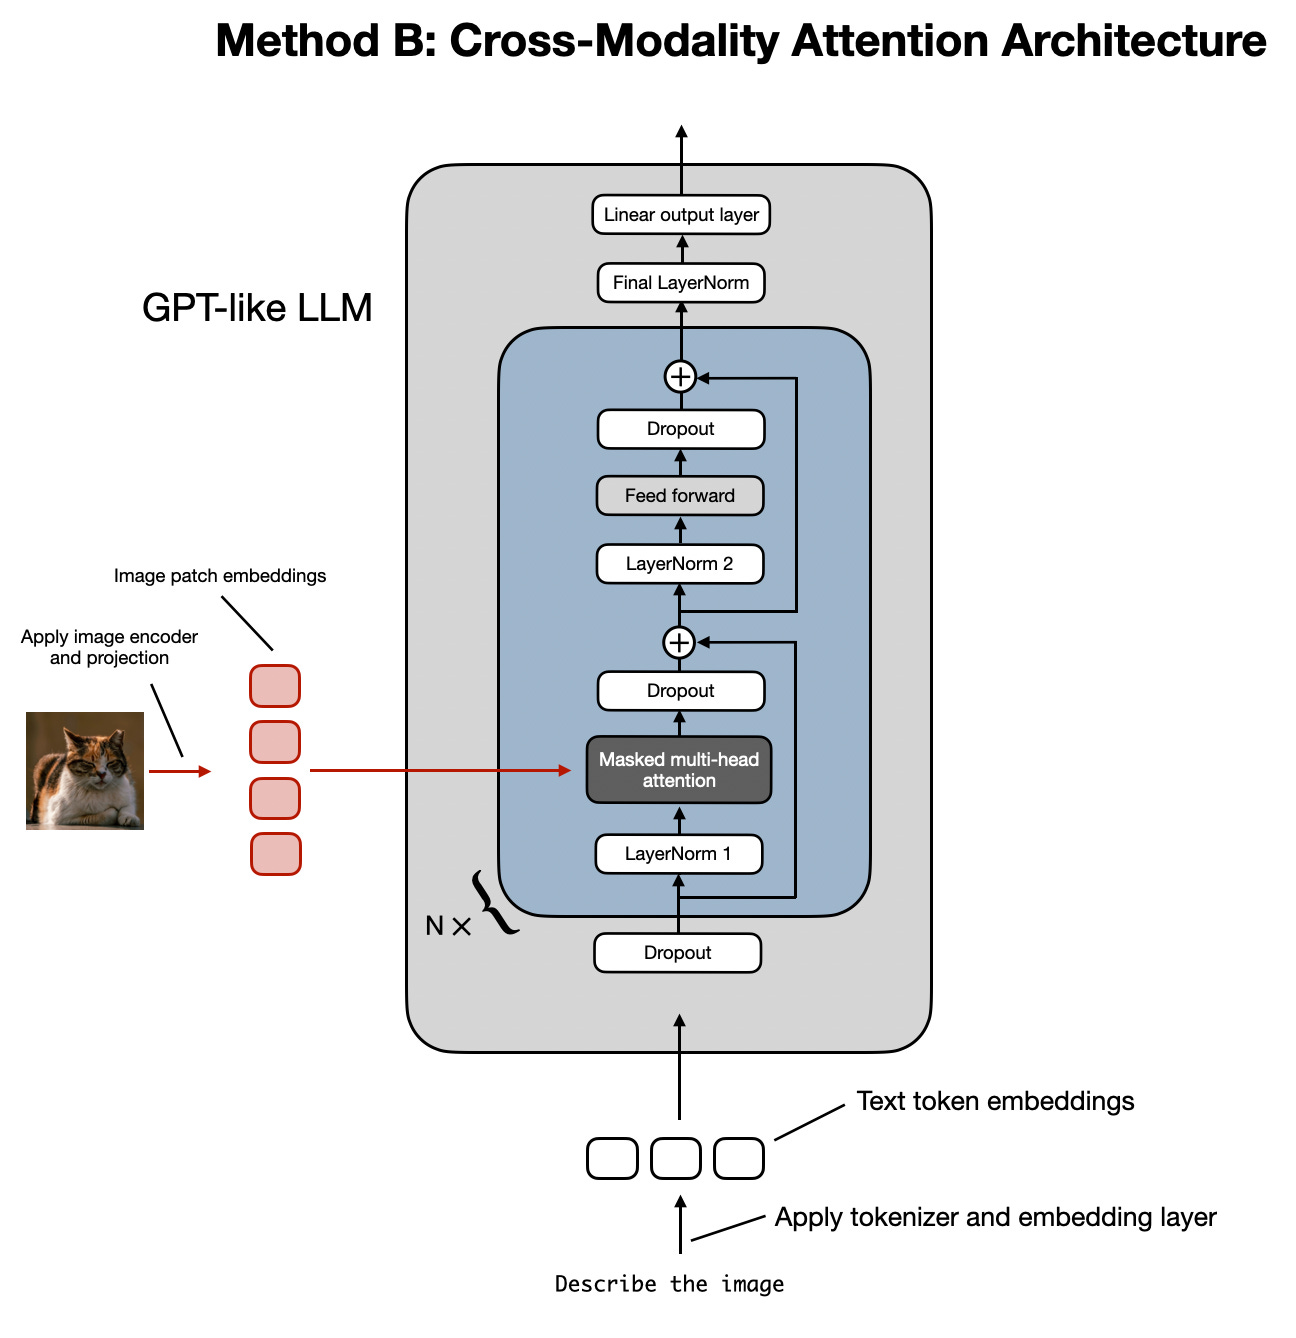
\includegraphics[width=0.85\textwidth]{img/pdz/17-cross-attention.jpg}
    \caption{Cross-attention \cite{raschka2024_multimodal_llms}.}
    \label{fig:Cross-attention}
\end{figure}

Cross-attention computes attention weights using queries from one sequence and key-value pairs from another. Given query matrix $Q$, key matrix $K$, and value matrix $V$

\begin{equation*}
    \text{Attention}(Q, K, V) = \text{softmax}\left(\frac{QK^{T}}{\sqrt{d_k}}\right)V
\end{equation*}

where:
\begin{itemize}
    \item $Q \in \mathbb{R}^{T_q \times d}$ are queries from the target modality (e.g., decoder text embeddings);
    \item $K, V \in \mathbb{R}^{T_k \times d}$ are keys and values from the source modality (e.g., encoder speech/image features);
    \item $d_k$ is the dimension of the key vectors;
    \item $T_q, T_k$ are token lengths for target and source sequences.
\end{itemize}

Multimodal fusion via dual attention for two modalities $A$ and $B$, cross-attention is computed independently:

\begin{equation*}
    H_{A} = \text{Attention}(Q, K_{A}, V_{A});
\end{equation*}

\begin{equation*}
    H_{B} = \text{Attention}(Q, K_{B}, V_{B}).
\end{equation*}

The fused representation is then computed as

\begin{equation*}
    H = \alpha H_{A} + (1 - \alpha)H_{B}
\end{equation*}

where $0 \leq \alpha \leq 1$ is a learnable fusion coefficient.


\section{Multimodal Embedding}

The rapid development of multimodal embedding architectures has significantly broadened the scope of retrieval systems, enabling richer representations across heterogeneous data sources. Early foundation models such as CLIP (2021) established a strong baseline for cross-modal embeddings by jointly training on 400 million image–text pairs and learning a shared embedding space for both modalities~\cite{radford2021clip}. CLIP’s dual-encoder design not only facilitated zero-shot image–text retrieval but also became a widely adopted backbone for subsequent multimodal systems. Building upon this foundation, recent research has extended embeddings to additional modalities and specialized domains.



Each input modality $m \in \{\text{text}, \text{audio}, \text{vision}\}$ is encoded into a latent vector using a modality-specific encoder
\begin{equation*}
    z_m = f_m(x_m; \theta_m)
\end{equation*}
where $x_m$ is the raw input of modality $m$, $f_m(\cdot)$ is the corresponding encoder (e.g., Transformer encoder for text, Conformer for audio, ViT for vision), and $\theta_m$ denotes its learnable parameters.


\begin{figure}[h!]
    \centering
    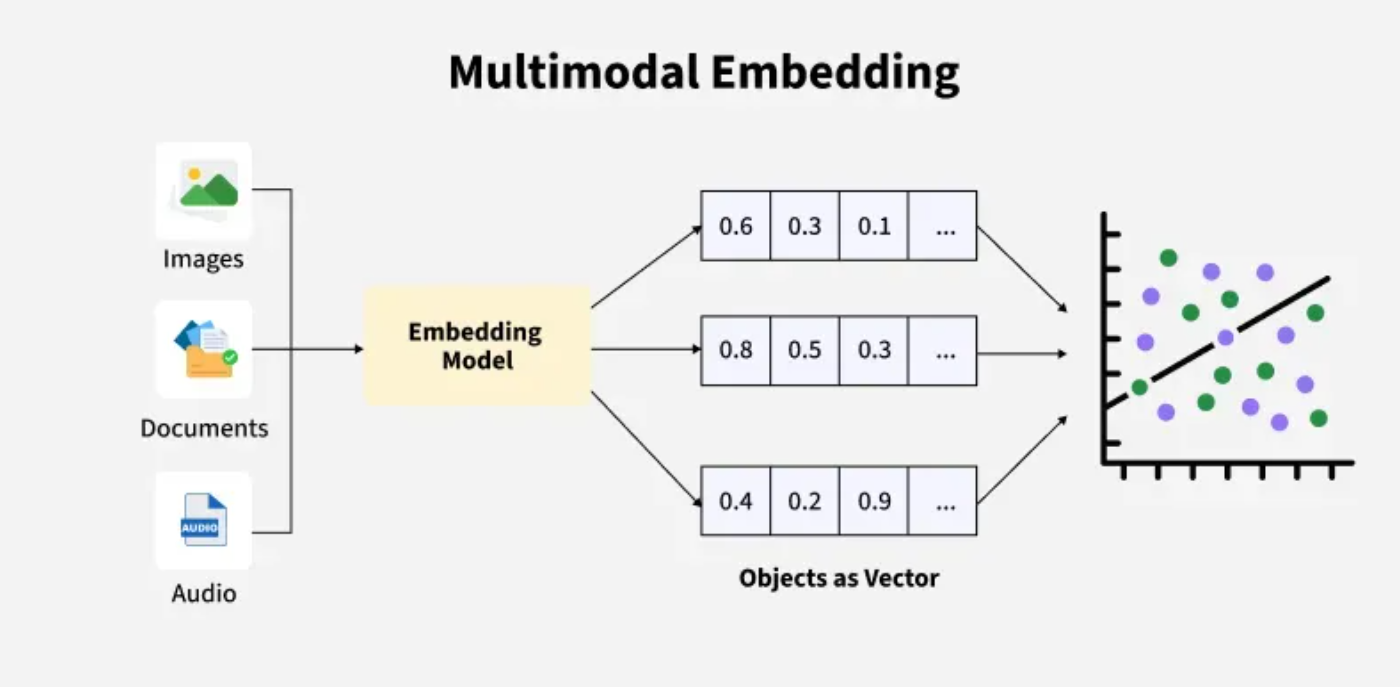
\includegraphics[width=0.9\textwidth]{img/pdz/05-multimodal-embedding.png}
    \caption{Multimodal embedding \cite{aiedge_multimodal_rag}.}
    \label{fig:Multimodal embedding}
\end{figure}


We fuse modality embeddings into a shared representation
\begin{equation*}
    z = g([z_{\text{text}}; z_{\text{audio}}; z_{\text{vision}}]; \phi)
\end{equation*}
where $[z_{\text{text}}; z_{\text{audio}}; z_{\text{vision}}]$ is the concatenation operator, $g([z_{\text{text}}; z_{\text{audio}}; z_{\text{vision}}])$ is a fusion network (e.g., MLP or cross-attention module), and $\phi$ denotes fusion parameters.

To align representations across modalities, we apply a contrastive loss
\begin{equation*}
    \mathcal{L}_{\text{contrast}} = -\sum_{i=1}^{N} \log
    \frac{\exp(\mathrm{sim}(z_i^{(a)}, z_i^{(t)}) / \tau)}
    {\sum_{j=1}^{N} \exp(\mathrm{sim}(z_i^{(a)}, z_j^{(t)}) / \tau)}
\end{equation*}
where $z_i^{(a)}$ and $z_i^{(t)}$ are the audio and text embeddings of paired sample $i$, $\mathrm{sim}(z_i^{(a)}, z_j^{(t)})$ is a similarity function (e.g., cosine similarity), $\tau$ is the temperature scaling factor, and $N$ is the batch size.


One line of progress has centered on multimodal large language models (MLLMs). These models, exemplified by LLaVA and LLaMA-2 Vision, can process both visual and textual input and have increasingly been repurposed for retrieval tasks. Lin et al. introduced MM-Embed, a multimodal LLM fine-tuned as a bi-encoder to support queries that combine images and text~\cite{lin2024mmembed}. While naïve multimodal LLM retrievers displayed modality biases, such as a tendency to over-prioritize text results, MM-Embed reduced these issues by incorporating modality-aware hard negatives during training. This adjustment enabled the model to achieve state-of-the-art performance on the M-BEIR benchmark, a multi-domain multimodal retrieval suite, and it even outperformed leading text-only retrievers on standard text-focused benchmarks~\cite{lin2024mmembed}. These findings demonstrate that, with careful fine-tuning, large multimodal models can function as powerful and general-purpose retrievers across different modalities.

Another noteworthy development is the emergence of unified multimodal embedding architectures. Meta AI’s ImageBind (2023) represents a landmark contribution by integrating six distinct modalities: images, video, text, audio, depth, thermal data, and IMU motion signals into a single shared embedding space~\cite{girdhar2023imagebind}. Crucially, ImageBind does not require explicit pairing for every modality. Instead, it learns a joint representation that enables flexible cross-modal retrieval; for instance, an audio recording of a lecture can retrieve a relevant diagram, or a video clip can be matched with its spoken description. This holistic framework signals the potential for future educational systems in which any form of input, whether speech, text, or image, can be used to locate semantically related content across heterogeneous media.

Beyond general-purpose models, domain-specific designs have also gained traction. Educational content frequently blends textual explanations with complex visual structures such as diagrams, charts, and mathematical formulas. To address this, models such as jina-embeddings-v4 (2025) have been proposed. With 3.8 billion parameters, this model integrates text and image data and supports both single-vector embeddings and multi-vector late-interaction embeddings~\cite{guenther2025jinaembeddingsv4}. It further incorporates task-specific adapters, trained via low-rank adaptation (LoRA), for applications including code search and question answering. The model achieves state-of-the-art results on text and multimodal retrieval benchmarks, particularly excelling in tasks involving visually dense content such as tables and lecture slides. To evaluate these capabilities, the authors introduced Jina-VDR, a benchmark for visually rich document retrieval, which underscores the critical importance of handling diagrams and mixed-media content in educational settings~\cite{guenther2025jinaembeddingsv4}.

Parallel efforts in industry have emphasized retrieval over multimodal documents such as PDFs and slides, which combine text layout with images. Nomic’s Embed Multimodal 7B (2025) exemplifies this trend by embedding interleaved text and images for retrieval-augmented generation over documents. While a formal paper for this model is not yet publicly available, industry documentation and benchmark reports indicate that this model achieved a new state-of-the-art on the ViDoRe–v2 visual document retrieval benchmark, recording an NDCG@5 of 62.7 and surpassing prior models by 2.8 points~\cite{nomic2025embedmultimodal}.

Finally, an important trend is the narrowing performance gap between multimodal and single-modal models. For example, the MM-Embed retriever, initialized from the NV-Embed text model, not only excelled at cross-modal retrieval but also outperformed strong text-only retrievers on the text-focused MTEB benchmark~\cite{lin2024mmembed}. This convergence suggests that training with multimodal data enhances the semantic richness of representations even for unimodal text tasks. Such results are particularly encouraging for educational contexts, where queries often combine textual and visual references, for example, a request to locate “the graph of X” alongside a written description.


\section{Retrieval-Augmented Generation}

\subsection{Historical Evolution of Retrieval-Augmented Generation}

\textbf{2017--2019: Pre-RAG foundations.}
Open-domain question answering prior to RAG largely followed a retrieve-then-read pipeline, where a sparse retriever fetched passages and a neural reader extracted answers. DrQA exemplified this architecture and established the modern baseline of TF-IDF/BM25 retrieval paired with a neural reader~\cite{chen2017drqa}. Neural methods then began to learn retrieval: ORQA jointly trained a dense retriever and reader from QA supervision, demonstrating that learned dual encoders could outperform purely sparse heuristics while remaining efficient at query time~\cite{orqa2019}. In parallel, kNN-LMs showed that a language model’s predictions can be conditioned on a non-parametric, external datastore during inference, anticipating the later concept of ``semi-parametric'' models that fluidly combine internal parameters with external memory~\cite{khandelwal2020knnlm}. Together, these developments set the stage for retrieval and generation to be tightly coupled rather than treated as disjoint stages.

\textbf{2020: Formalizing retrieval-augmented generation.}
REALM introduced end-to-end differentiable retrieval during pretraining so that a masked-LM objective could backpropagate through a large document index, demonstrating that external, updateable knowledge could be learned and consulted by the LM at scale~\cite{realm2020}. Shortly afterward, RAG combined a dense retriever (DPR) with a sequence-to-sequence generator (BART), training the entire model so that gradients update both retriever and generator. This ``general-purpose fine-tuning recipe'' showed that a medium-sized LM augmented with learned retrieval can outperform substantially larger parametric-only models on knowledge-intensive tasks~\cite{lewis2020rag}.

\textbf{2021--2022: Stronger Retrievers, Multi-Document Reasoning, and Lighter Readers}

Dense retrieval advanced on several fronts: RocketQA introduced denoised hard negatives and cross-batch training \cite{rocketqa2021}; RocketQAv2 refined knowledge distillation from cross-encoders to bi-encoders for latency-aware quality \cite{rocketqa2_2021}. Retriever-specific pretraining (Condenser) made language-model pretraining explicitly serve dense retrieval \cite{condenser2021}, while unsupervised contrastive pretraining (Contriever) yielded robust, domain-transferable retrievers without labels \cite{contriever2021}. Scaling T5 dual encoders (GTR) further improved zero-shot transfer \cite{gtr2021}. Beyond bi-encoders, late-interaction architectures (ColBERTv2) compressed token-level matching to make interaction models practical at scale, often used as a re-ranking stage \cite{colbertv2_2021}. In sparse-dense hybrids, SPLADE and SPLADE-v2 showed that learned sparsity pairs naturally with dense vectors; hybrid fusion became a ``default'' for out-of-distribution robustness \cite{splade2021, spladev2_2021}.

At the same time, RAG pipelines learned to retrieve multiple supporting documents: EMDR pushed learning signals across the retrieve$\rightarrow$read boundary with an EM-style objective \cite{emdr2021}, and MDR operationalized multi-hop chains of evidence for compositional questions \cite{mdr2020}. On the reader side, Fusion-in-Decoder (FiD) became a standard for fusing many passages, while KG-FiD injected graph structure and GNN-based re-ranking to pass only high-value evidence to the decoder \cite{fid2020,kgfid2021}. FiD-Light then reduces context while constraining encoder$\rightarrow$decoder flow and source-aware re-ranking, improving the accuracy–latency Pareto frontier \cite{fidlight2022}. Retrieval-on-the-fly matured via RETRO, which matched the quality of a model roughly $25\times$ larger by consulting a massive index during generation, reinforcing the promise of semi-parametric scaling \cite{retro2021}.

Bridging retriever and generator also simplified: Retrieval-as-Attention (ReAtt) folded retrieval into a single transformer trained end-to-end \cite{reatt2022}, and Re2G unified initial retrieval, re-ranking, and generation in one seq2seq framework \cite{re2g2022}. Meanwhile, RAG-oriented query reformulation rose to prominence: GAR enriched queries with generated contexts; Self-Ask and ReAct interleaved decomposition/reasoning with search; WebGPT introduced browser-assisted QA with feedback; and HyDE generated ``hypothetical documents'' to boost first-stage recall---techniques that remain plug-and-play modules in modern RAG stacks \cite{gar2021, selfask2022, react2022, webgpt2021, hyde2022}.

\textbf{2023--2024: From fixed pipelines to adaptive, verifiable, and structure-aware systems.}

Active/adaptive retrieval made when and what to retrieve a learned, closed-loop decision. FLARE triggered retrieval mid-decoding when uncertainty spiked; Adaptive-RAG learned to route among no-retrieval vs. single- or multi-step strategies; SEAKR and DRAGIN dynamically chose whether/what to retrieve conditioned on evolving information needs, cutting cost while improving grounding \cite{flare2023, adaptive_rag2024, seakr2024, dragin2024}. Robustness moved from “more context fewer hallucinations” to controlling what gets used. SELF-RAG alternated retrieve→generate→critique cycles; CRAG filtered low-quality evidence or refused to answer; CoV-RAG added a chain-of-verification to revise queries/answers; and independent analysis documented the tug-of-war between an LM’s priors and retrieved facts motivating verification-aware decoding \cite{selfrag2023, crag2024, covrag2024, lmpriors2024}.

Context selection and compression became first-class: RankRAG instruction-tuned a single LLM to rank contexts and generate answers, while LLMLingua and a 2024 survey systematized aggressive yet faithful compression to stay within prompt budgets \cite{rankrag2024, llmlingua2023, compression2024}. Retrieval broadened to multi-source/agentic settings: AU-RAG introduced source-aware routing among heterogeneous corpora (web/wiki/vertical DBs), and MSPR learned policies for which source to consult and how much to retrieve \cite{au_rag2024, mspr2024}. Structure-aware retrieval emerged: GraphRAG and GRAG indexed entities/communities and retrieved subgraphs instead of IID chunks, enabling corpus-level synthesis and multi-hop reasoning over relationships \cite{graphrag2024, grag2024}. Finally, long-context LLMs met RAG: LongRAG combined long retriever + long reader to keep fewer but larger 4K-token units, and self-routing decided between long-context reading and targeted RAG per query \cite{longrag2024, selfroute2024}.

\textbf{2025: Agentic control, standardized modules, faithful decoding, evaluation, and memory.}
By 2025, “Agentic RAG” is crystallized in surveys that codify reflection, planning, tool use, and multi-agent collaboration as control loops over retrieval; HopRAG exemplifies logic-guided hops over a passage graph before generation \cite{survey_agentic2025, survey_reasoning_agentic2025, hoprag2025}. Complementary surveys standardize the pipeline into four tunable modules (1) retrieval optimization, (2) context processing (re-rank/filter/compress), (3) generation optimization (faithfulness/citation-aware decoding), and (4) evaluation/monitoring collecting robustness and efficiency tactics in each \cite{knowledge_oriented_survey2025, architectures_survey2025}. Generation now explicitly enforces use of evidence: FaithfulRAG models LM-vs-retrieval conflicts and inserts self-thinking before decoding; ReCLAIM constrains decoding with per-sentence citations; CiteFix repairs/validates citations post-hoc; and new studies plus CiteBench/CiteEval move toward principled attribution metrics \cite{faithfulrag2025, reclaim2024, citefix2025, source_attribution2025, citeeval2025}. Evaluation became first-class: ARES provides automated judge-based scoring of context relevance, answer faithfulness, and answer relevance; a 2025 survey consolidates datasets/metrics including abstention and multi-hop fidelity; and competitions like “live RAG” benchmarks (e.g., RAGtifier) standardize end-to-end evaluation on time-varying corpora \cite{ares2024, survey_eval2025, ragtifier2025}.

Finally, RAG is reframed as memory and continual learning: HippoRAG-2 strengthens associative, graph-traversal memory; MemoRAG proposes a dual-system (light long-range LM for global memory + expressive LM for final answers); and agent-memory systems (Mem0, MIRIX, MemOS) treat persistent, structured memories as read/write stores that RAG can consult blurring retrieval, memory, and learning with provenance and versioning \cite{hipporag2_2025, memorag2024, mem0_2025, mirix2025, memos2025}.

\subsection{mRAG: The Convergence}
\textbf{Pre-RAG signals for vision–language tasks.}  
Before mRAG (mRAG) was named, factual VQA exposed the limits of image-only reasoning. “Straight to the Facts” explicitly learned KB retrieval for VQA, and OK-VQA required outside knowledge, catalyzing retrieval-style VQA where images must be grounded in world facts \cite{marino2019okvqa}.

\textbf{2022–2023: Early mRAG patterns.}  
Two threads converged. First, VQA pipelines adopted RAG-style structures: TRiG translated images to text, retrieved passages, and answered purely in NL space pragmatically reusing text-RAG infrastructure \cite{gao2022trig}; and differentiable retrieval models, such as entity-focused dense passage retrieval, improved retrieval for OK-VQA \cite{wu2022entityvqa}. Second, cross-modal embeddings provided the retrieval substrate: CLIP and ALIGN learned shared image–text spaces enabling text-image nearest-neighbor search at scale. REVEAL then pushed end-to-end retrieval-augmented visual-language pre-training with a multi-source multimodal memory, tying a retriever and generator together during pretraining \cite{hu2023reveal}.  

In generation, retrieval-augmented captioning appeared: Ramos et al. retrieved captions for stronger descriptions, and EVCap added an external “visual-name” memory to keep captions up-to-date in open-world settings. FLMR aligned vision encoders to text retrievers and used multi-dimensional embeddings to capture finer-grained query–document relevance, improving cross-modal matching. Across these systems, the unit of retrieval was predominantly textual (captions/Wikipedia/OCR), even when the queries were visual; the fusion mechanism typically concatenated retrieved text as extra tokens to a VL encoder/decoder.

\textbf{2024: Maturation – better retrieval and fusion for VLMs, and broader modality bindings.}  
VisRAG explicitly treats visually rich documents as first-class evidence by combining OCR text with visual region cues for retrieval and grounding, bridging VQA-style methods to real-world documents \cite{yu2024visrag}. RAVEN frames retrieval-augmented VLM fine-tuning as a general recipe across tasks \cite{rao2024raven}, while DIR improves both image→text retrieval and the utilization of retrieved text for more complete visual understanding.

In parallel, ImageBind shows a single embedding space for six modalities (image, text, audio, depth, thermal, IMU), widely cited to justify one-index, cross-modal retrieval for mRAG systems that must unify heterogeneous educational assets (slides, lab audio, sensor feeds) \cite{girdhar2023imagebind}.

\textbf{2025: Advanced mRAG – domains, video, documents, and built-in retrieval.}  
Domain‑specific mRAG shows substantial gains when retrieval and verification are tuned to the domain. In remote sensing, RS‑RAG integrates satellite imagery with world knowledge through a multimodal index and reports large improvements on captioning/classification/VQA \cite{wen2025rsrag}.  

Video becomes a first‑class citizen: Multimodal Retrieval‑Augmented Generation systems unify information across text, image, table, and video modalities in a single pipeline \cite{drushchak2025unified}.  

Evaluation and instruction‑tuning keep pace. A recent survey consolidates components, tasks, and datasets for mRAG and argues empirically that mRAG reduces hallucinations on visually grounded queries compared to text‑only RAG \cite{mei2025survey}.



\subsection{Pipeline}

\begin{figure}[h!]
    \centering
    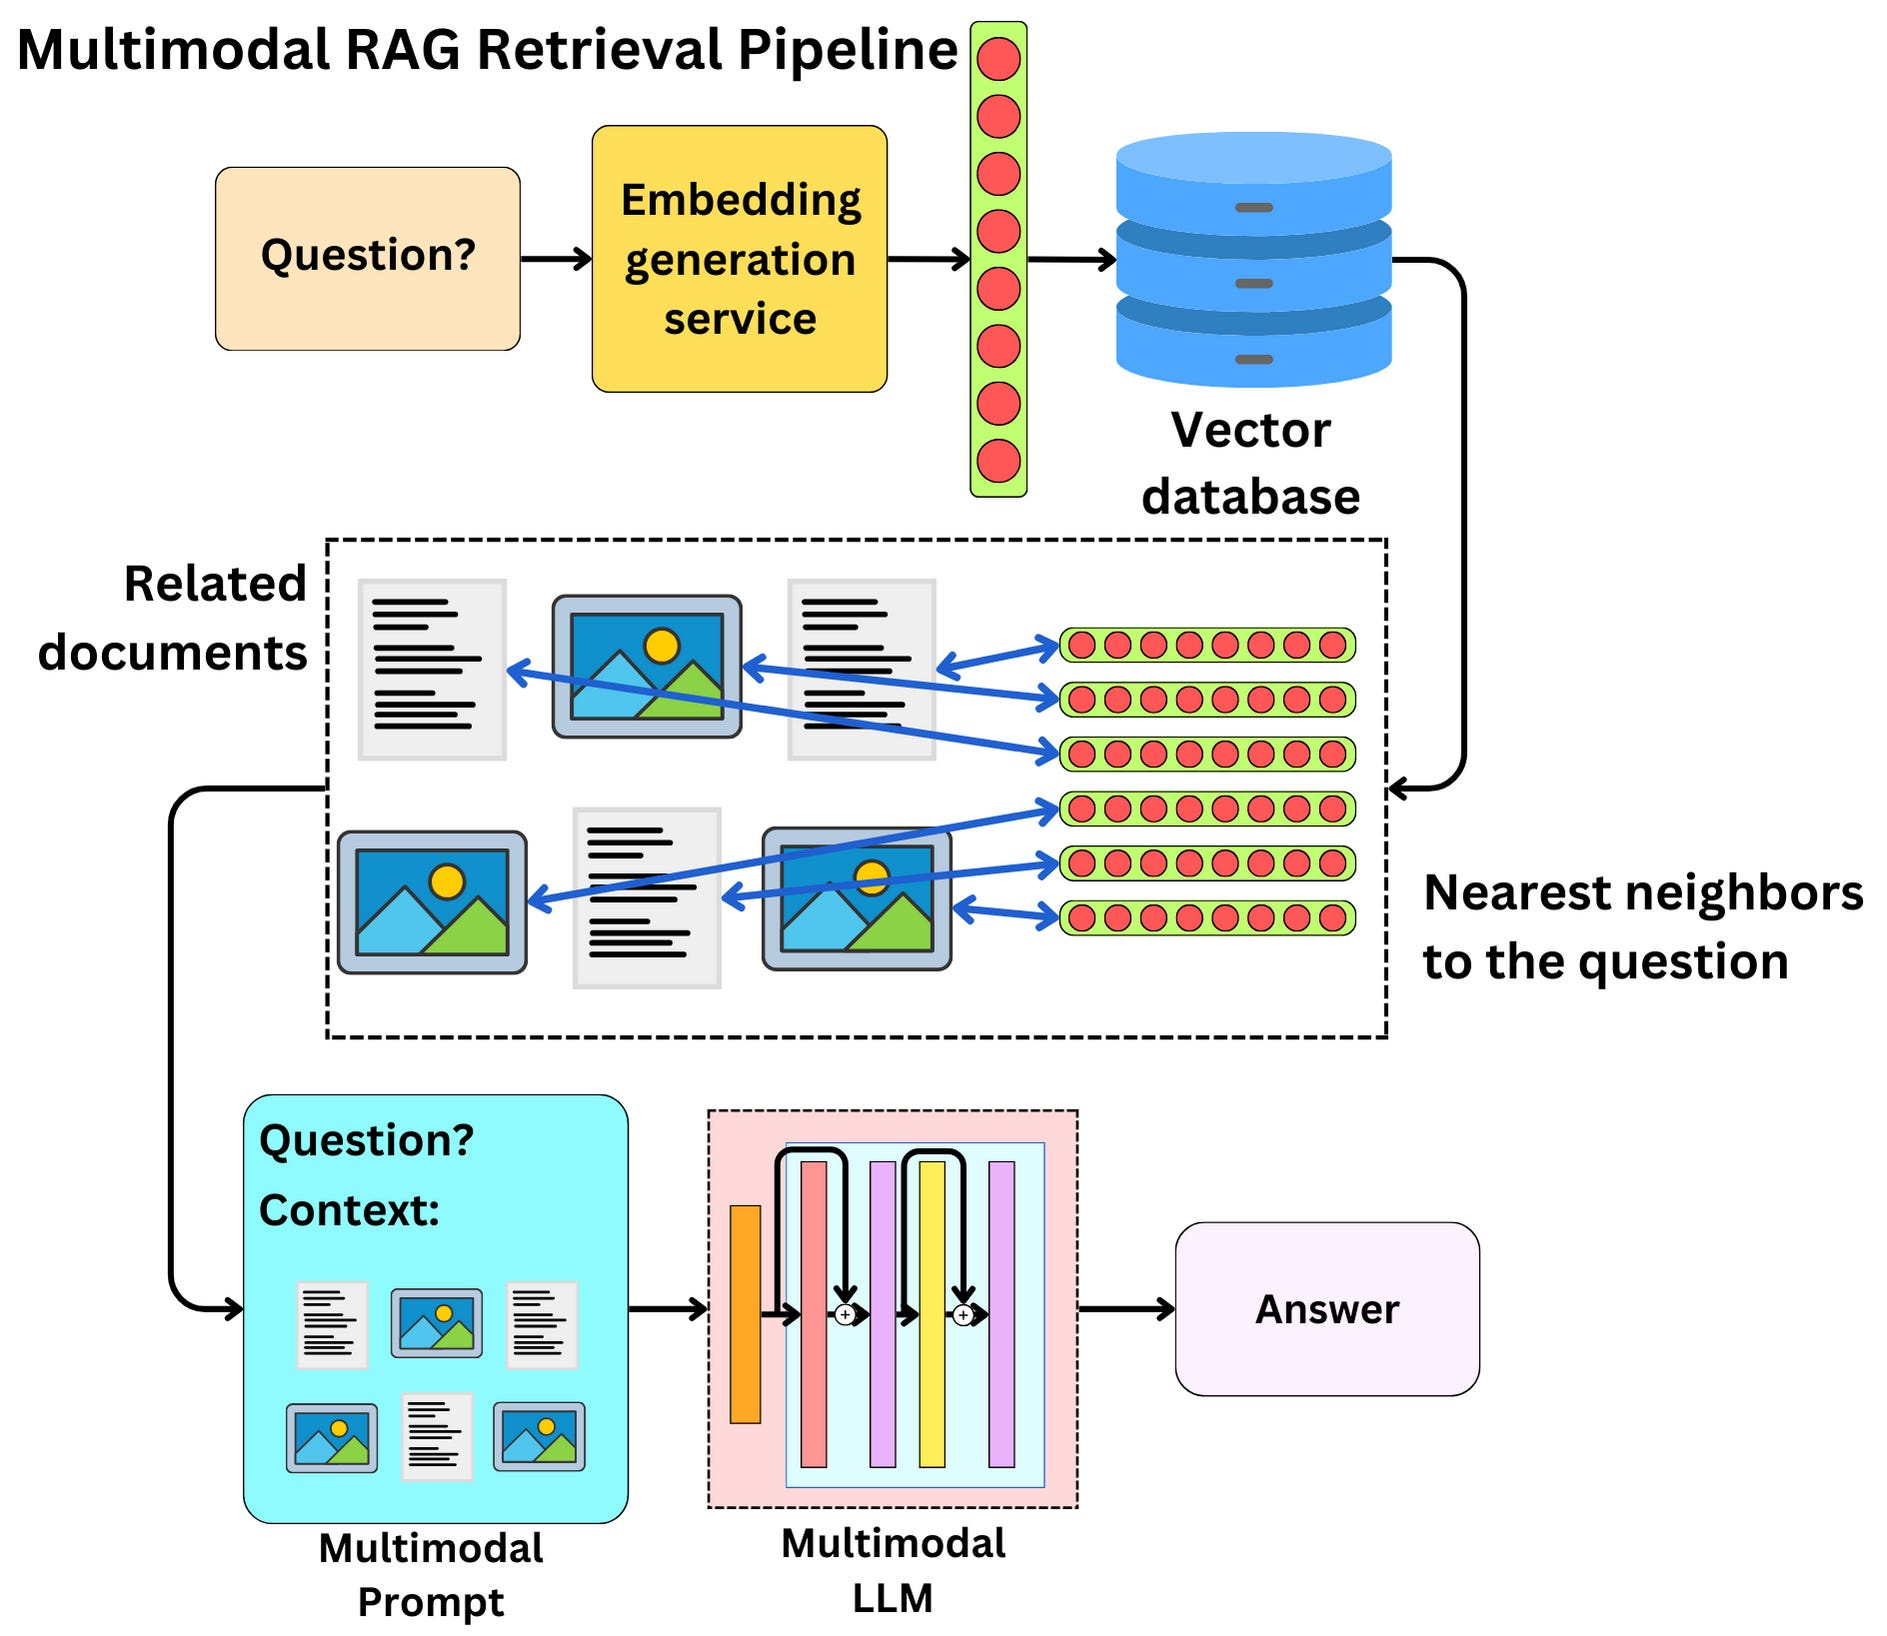
\includegraphics[width=0.9\textwidth]{img/pdz/02-multimodal-rag-pipeline.jpg}
    \caption{mRAG pipeline \cite{aiedge_multimodal_rag}.}
    \label{fig:mRAG pipeline}
\end{figure}

The RAG pipeline integrates retrieval mechanisms with generative language models to produce accurate and contextually grounded outputs. The process begins with query vectorization, where the user input is encoded into a high-dimensional vector representation using models such as BERT or Sentence Transformers. This query vector is then matched against a pre-indexed vector database to identify semantically similar entries, allowing the system to retrieve the most relevant documents or passages~\cite{karpukhin2020dense, lewis2020rag}.
After retrieval, the selected data may undergo preprocessing steps for example, summarization, filtering, or restructuring to ensure compatibility with the downstream language model. The processed information is then incorporated into the input context of a large language model (LLM), enabling it to generate responses that combine the retrieved evidence with its own pre-trained knowledge~\cite{izacard2021leveraging}.

The Retrieval-Augmented Generation architecture consists of two primary modules: the retriever and the generator. The retriever is responsible for identifying relevant documents or passages from an external knowledge source. It typically operates using methods such as sparse retrieval (e.g., BM25), dense vector retrieval based on embedding similarity, or hybrid/neural retrieval models~\cite{lewis2020rag, luan2021sparse_dense}. These techniques allow the system to efficiently search large-scale corpora and return the most semantically relevant information.

The generator then consumes both the user query and the retrieved context to produce the final output. Modern RAG systems usually rely on transformer-based language models, which condition their decoding process on the retrieved evidence to ensure that the generated response is grounded in factual information and remains aligned with the input query~\cite{lewis2020rag, izacard2022rag_sequence}.

By combining retrieval with generation, RAG reduces hallucination rates, improves factual accuracy, and enables the model to access up-to-date or domain-specific knowledge without needing to retrain the entire language model. This makes RAG a practical and scalable solution for knowledge-intensive tasks in machine learning and natural language processing~\cite{lewis2020rag, izacard2021leveraging, gao2023rag_survey}.



Moreover, recent advances in mRAG further expand its capabilities. For example, mRAG systematically explores different modality configurations (text, image, video, table), retrieval strategies, reranking, and how to integrate retrieved evidence into generation, achieving significant improvements without fine-tuning~\cite{hu2025mrag}. Another variant, HM-RAG, proposes a hierarchical multi-agent architecture where multiple retrieval agents (text, graph, web) work collaboratively and feed into a decision agent, improving answer accuracy on multimodal benchmarks~\cite{liu2025hmrag}. In visually rich QA settings, models like mR²AG adapt retrieval dynamically and reflect on the relevance of retrieved multimodal evidence to guide generation~\cite{zhang2024mr2ag}. These innovations illustrate that RAG combined with multimodal retrieval and generation is becoming increasingly powerful   especially for complex, knowledge-intensive, multimodal educational applications.

\subsection{Retrieval}

Sparse retrieval models represent the classical approach to information retrieval, mapping texts into high-dimensional, sparse vectors based on lexical features~\cite{robertson2009probabilistic, formal2021splade}. These methods, such as TF-IDF and BM25, rely on keyword frequency statistics to determine relevance. The resulting vectors excel at exact keyword matching, making them highly effective and interpretable for queries where specific terms are crucial~\cite{robertson2009probabilistic}. More advanced models like SPLADE are also based on this sparse representation paradigm~\cite{formal2021splade}. The underlying scoring function for these models can typically be expressed as an inner product between the sparse vector representations of the query and the document. Retrieval is traditionally performed efficiently using an inverted index~\cite{formal2021splade}. However, they can struggle with keyword mismatches, which means they cannot effectively handle semantic similarity where the exact keywords are not present in the document~\cite{formal2021splade}.


\begin{figure}[h!]
    \centering
    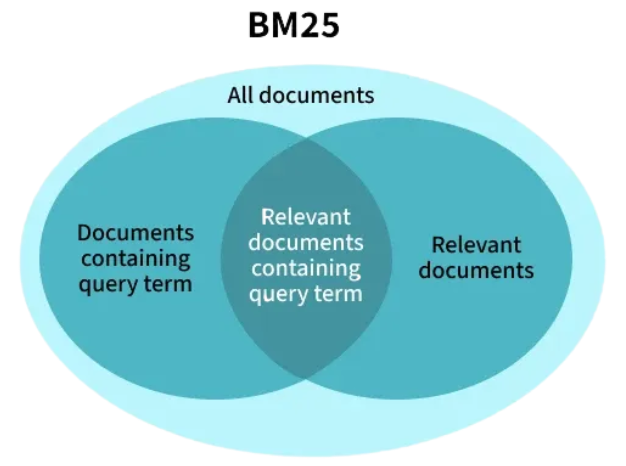
\includegraphics[width=0.6\textwidth]{img/pdz/16-bm25.png}
    \caption{BM25 \cite{geeksforgeeks_bm25}.}
    \label{fig:BM25}
\end{figure}


Dense retrieval emerged with the advent of deep learning, employing models to learn low-dimensional, dense vector representations that capture semantic meaning~\cite{karpukhin2020dense}. This approach, often implemented as a dual encoder, maps queries and documents into a shared embedding space where semantic similarity corresponds to vector proximity, typically measured by inner product~\cite{karpukhin2020dense}. Models like BERT-based DPR and SPECTER2 (for scientific documents) are trained to encode contextual information, allowing them to excel at semantic matching even when keywords differ~\cite{karpukhin2020dense, singh2022scirepeval}. These dense vectors can be indexed for efficient large-scale retrieval using Approximate Nearest Neighbor Search (ANNS) algorithms, with graph-based methods like Hierarchical Navigable Small World (HNSW) being particularly effective~\cite{malkov2016efficient}. While powerful for semantic understanding, dense models can lack the precision needed for exact term matching. Furthermore, theoretical and empirical analyses show that the capacity of fixed-length dense encoders can be limited, with performance potentially degrading as document length increases. This is because longer documents introduce smaller normalized margins between relevant and non-relevant items, requiring a larger encoding dimension to maintain fidelity with sparse models~\cite{formal2021splade}.

To leverage the complementary strengths of both paradigms, hybrid retrieval has become a widespread and effective practice, particularly in systems like Retrieval-Augmented Generation~\cite{li2020rag}. The core idea is to fuse sparse and dense signals to enhance both effectiveness and robustness~\cite{formal2021splade, karpukhin2020dense}. A simple yet effective approach is to linearly combine the scores from separate sparse and dense retrievers~\cite{formal2021splade, karpukhin2020dense}. Another common strategy is the two-route method, where sparse and dense searches are conducted separately and the results are merged~\cite{formal2021splade}. However, this increases system complexity and can compromise accuracy, as the top hybrid results may not be in the top-k results of either individual system~\cite{formal2021splade}. A more advanced approach is to build a unified index for concatenated dense-sparse hybrid vectors. This presents two key challenges: (1) the significant difference in data distribution between dense and sparse vectors makes it difficult to combine them optimally, potentially hurting accuracy; and (2) the high dimensionality and computational cost of sparse vectors can degrade retrieval efficiency. To address this, recent work proposes methods like distribution alignment (using pre-sampling to determine optimal fusion weights) and an adaptive two-stage computation strategy (initially using only dense distances for coarse search and later refining with hybrid distances) to improve both accuracy and speed~\cite{formal2021splade, iida2022unsupervised}.

Once embeddings have been generated, the retrieval module identifies and returns the most relevant
documents for a given query. In a RAG pipeline, this step is essential because it supplies the language
model with context that guides accurate response generation. Formally, given a query $q$ in language $x$,
the retriever returns a document $d$ in language $y$ (which may or may not match $x$) from a corpus
$D_y$. The retrieval function $f_n^\ast$ may be implemented using dense, lexical, or multi-vector retrieval
methods~\cite{chen2024bge}
\[
    d_y \leftarrow f_n^\ast(q_x, D_y).
\]

\textbf{Dense Retrieval:} A query $q$ is encoded into hidden states $H_q$ using a text encoder. The representation of the query
is the normalized hidden state of the special token \texttt{[CLS]}
\[
    e_q = \mathrm{norm}(H_q[0]).
\]
Similarly, for a passage $p$
\[
    e_p = \mathrm{norm}(H_p[0]).
\]
Relevance is computed as the inner product
\[
    s_{\mathrm{dense}} = \langle e_p, e_q \rangle.
\]

\textbf{Lexical Retrieval:} For each term $t$ in the query
\[
    w_{q t} = \mathrm{ReLU}(W_{\mathrm{lex}}^\top H_q[i]),
\]
and similarly for a passage
\[
    w_{p t} = \mathrm{ReLU}(W_{\mathrm{lex}}^\top H_p[i]).
\]
Where:
\[
    W_{\mathrm{lex}} \in \mathbb{R}^{d \times 1};
\qquad
\mathrm{ReLU}(x) = \max(0, x).
\]

\textbf{Multi-vector Retrieval:} Both queries and passages are represented using multiple vectors.

\[
    E_q = \mathrm{norm}(W_{\mathrm{mul}}^\top H_q),
    \qquad
    E_p = \mathrm{norm}(W_{\mathrm{mul}}^\top H_p),
\]
where:
\[
    W_{\mathrm{mul}} \in \mathbb{R}^{d \times d},
\]
and the normalization function is applied column-wise.


\subsection{Rerankers}

Rerankers, commonly implemented as cross-encoders, refine search results by jointly encoding a query--document pair to compute a relevance score. Unlike bi-encoders, which independently embed queries and documents into fixed-length vectors, rerankers leverage full token-level interactions, enabling more precise semantic matching. They are typically integrated into two-stage retrieval pipelines, where the first-stage retriever generates candidate documents and the reranker refines their ordering to achieve higher accuracy.


\begin{figure}[h!]
    \centering
    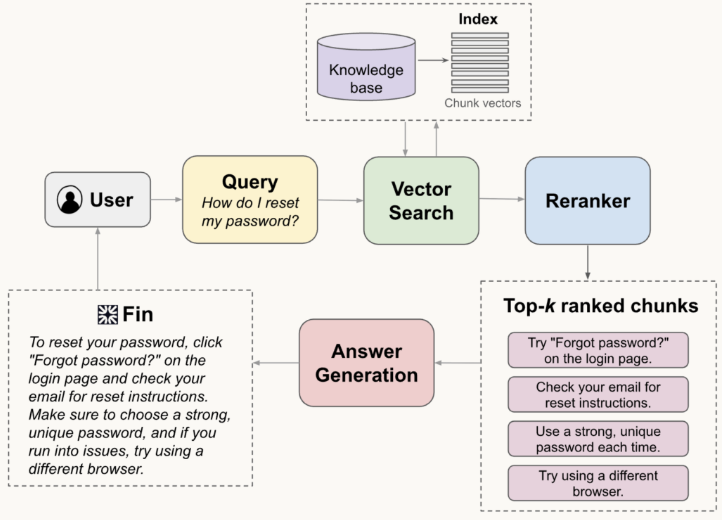
\includegraphics[width=1\textwidth]{img/pdz/16-reranker.png}
    \caption{Reranker \cite{together2024_rerank_llamarank}.}
    \label{fig:Reranker}
\end{figure}

Rerankers model token-level cross-attention between the query and document, allowing nuanced reasoning such as entity correspondence, negation detection, factual verification, semantic alignment, and multi-hop reasoning. This yields high relevance precision, especially in long-form document retrieval, question answering, and factual verification tasks.

Rerankers are computationally expensive and therefore operate on a narrowed candidate set rather than the full corpus. This architecture is decomposed as follows:
\begin{itemize}
    \item Stage 1 (Efficient Retrieval): A bi-encoder or sparse retriever (e.g., BM25, DPR, ColBERT) selects the top-$k$ candidates efficiently using vector similarity or lexical matching.
    \item Stage 2 (Precision Reranking): A cross-encoder transformer takes $(q, d)$ jointly as input and outputs a scalar relevance score used to reorder the candidate list.
\end{itemize}

This separation balances scalability and accuracy: fast retrieval reduces search space, while rerankers optimize precision at the top ranks.


Bi-encoders compute representations independently:
\[
\text{doc} \rightarrow \mathbf{v}_d \in \mathbb{R}^d, \quad \text{query} \rightarrow \mathbf{v}_q \in \mathbb{R}^d
\]
Similarity is computed via vector metrics (e.g., dot product), which is efficient but compresses document semantics into a single vector without query-context information.

Rerankers instead compute relevance jointly:
\[
\text{Reranker}(q, d) \rightarrow \text{score} \in \mathbb{R}
\]
This allows the model to consider local alignments and contextual dependencies, improving performance on tasks requiring fine-grained semantic reasoning. However, the computation happens online for each query-document pair and cannot be precomputed.


Bi-encoder indexing is performed offline, and inference requires only a single query encoding followed by approximate nearest neighbor search. This enables millisecond-scale retrieval over large corpora.

Rerankers require full transformer inference for every candidate document:
\[
q + d \rightarrow \text{Transformer} \rightarrow \text{score}
\]
As corpus size grows, reranking becomes increasingly expensive. For example, reranking 40M documents with a BERT-based model on a V100 GPU may require over 50 hours per query, while bi-encoder retrieval completes in under 100 ms. Thus, rerankers are typically applied to only 10–1000 candidates rather than the full index.

\subsubsection*{Impact on Retrieval Quality}

Empirically, rerankers consistently improve performance on metrics such as Recall and Mean Reciprocal Rank. They are particularly effective in:
\begin{itemize}
    \item open-domain question answering
    \item legal and biomedical retrieval where precision is critical
    \item multi-step reasoning and claim verification
    \item reranking passages in RAG pipelines for LLM-based generation
\end{itemize}

Their ability to leverage token-level attention enables them to differentiate between subtle semantic variations (e.g., contradiction vs. support), which bi-encoders often fail to distinguish due to embedding compression.

\begin{itemize}
    \item \textbf{Bi-encoders:} Scalable retrieval with precomputed embeddings, but limited by lossy compression.
    \item \textbf{Rerankers:} High precision via joint computation, but expensive at query time.
    \item \textbf{Two-stage retrieval:} Combines scalability and precision, forming the standard architecture for modern retrieval systems.
\end{itemize}


Early neural reranking approaches focused on applying cross-encoders to improve lexical retrieval methods such as BM25. ColBERT-v2 introduced a hybrid architecture combining late interaction with approximate vector search, enabling high recall with reduced latency while preserving token-level semantics \cite{colbertv2}. Unlike traditional bi-encoders, ColBERT performs interaction at inference time but maintains efficiency through compressed token embeddings and multi-stage pruning.

MonoT5 advanced reranking by framing document relevance as a sequence-to-sequence task using a generative T5-based model \cite{monot5}. Instead of predicting similarity scores directly, MonoT5 reformulates ranking as a text generation problem, allowing language models to leverage pretraining objectives for improved relevance judgment. This approach demonstrated state-of-the-art performance on MS MARCO and BEIR benchmarks, highlighting the effectiveness of generative rerankers.

More recent developments explore instruction-tuned and task-adaptive reranking. TART \cite{tart} proposes a unified instruction interface that enables strong zero-shot retrieval across numerous downstream datasets without dataset-specific finetuning. By conditioning reranking on natural language task descriptions, TART generalizes beyond traditional supervised ranking settings.

Recent LLM-based methods push reranking further by using large language models for alignment, reasoning, and verification. RankGPT \cite{rankgpt} employs ChatGPT as a reranker through a listwise ranking formulation, enabling the model to score and reorder multiple documents simultaneously. Rather than computing independent pairwise scores, RankGPT uses global contextual reasoning across the candidate set to mitigate position bias and improve ranking coherence.

These methods collectively highlight two major trends in reranking research: (1) scaling token-level interaction while maintaining computational feasibility (e.g., ColBERT-v2), and (2) leveraging generative and instruction-tuned LLMs to improve reasoning and generalization (e.g., MonoT5, TART, RankGPT). In modern RAG pipelines, rerankers increasingly serve not only as precision filters but also as semantic evaluators supporting long-context reasoning, multi-hop retrieval, and factual consistency.

\subsection{Augmentation}

\begin{figure}[h!]
    \centering
    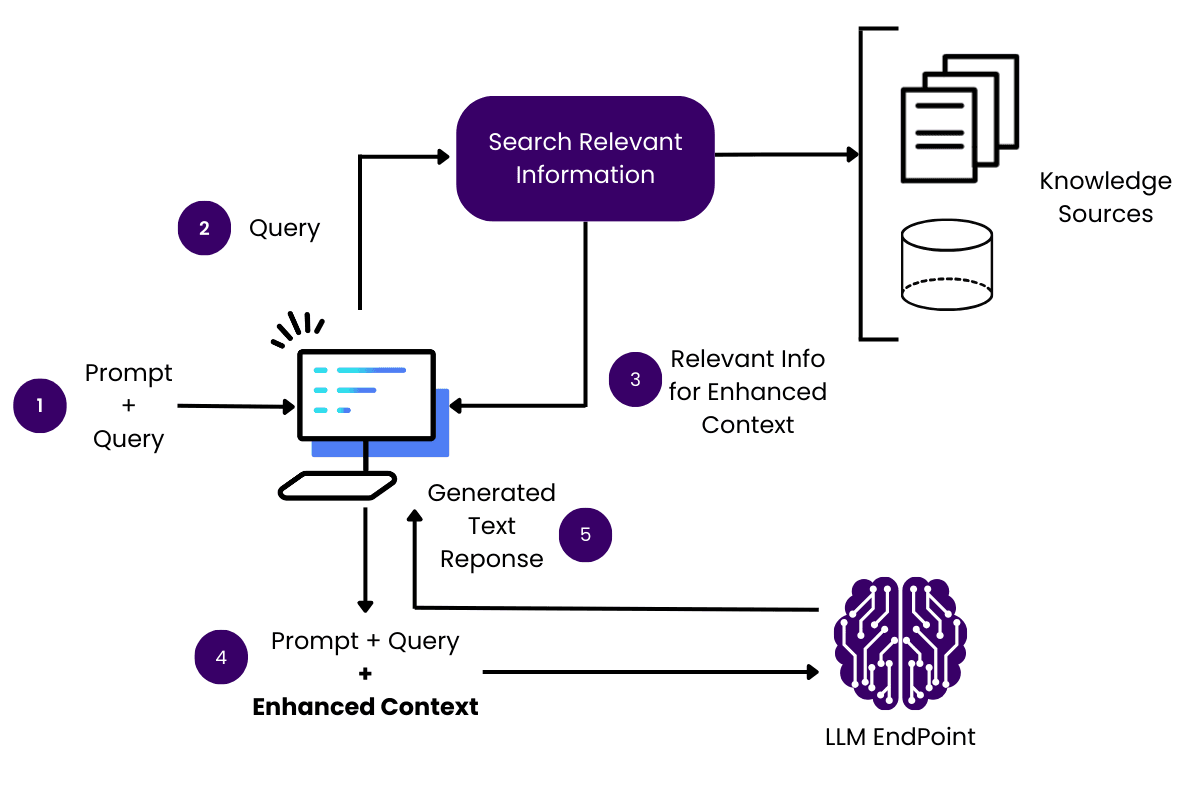
\includegraphics[width=0.9\textwidth]{img/pdz/07-augmentation.png}
    \caption{Augmentation \cite{obot_rag_guide}}
    \label{fig:Augmentation}
\end{figure}

Augmentation in Retrieval-Augmented Generation refers to the process of expanding or transforming retrieved knowledge prior to generation, enabling the model to leverage richer, more structured evidence. Unlike raw retrieval pipelines, augmentation enhances retrieved data through summarization, compression, restructuring, or synthetic expansion, improving relevance and reducing noise \cite{yoon2024compact, asai2023selfrag}.

Given a retrieved document set $D = \{d_1, \dots, d_k\}$, augmentation produces a transformed set $D' = \mathcal{A}(D)$ where $\mathcal{A}$ is an augmentation operator such as summarization, chunk merging, entity extraction, or reasoning-based synthesis. Formally:
\[
D' = \mathcal{A}(D) = \{ a_1, \dots, a_m \}, \quad m \leq k \; \text{or} \; m \geq k,
\]
where each augmented element $a_i$ may be compressed, reformatted, or newly generated from retrieval.

To preserve semantic coverage while reducing redundancy, augmentation can be framed as an optimization objective:
\[
\max_{D'} \; \text{Rel}(D', q) - \lambda \, \text{Redund}(D'),
\]
where $\text{Rel}$ measures relevance to query $q$ and $\text{Redund}$ quantifies informational overlap.

A common augmentation strategy is active document compression, where generative models summarize retrieved passages while preserving answer-critical semantics \cite{yoon2024compact}. This can be modeled as:
\[
a_i = \arg\max_{a} P(a \mid d_i, q),
\]
and scored using a utility function:
\[
s(a_i, q) = \alpha \cdot \text{Sim}(a_i, q) + \beta \cdot \text{Coverage}(a_i, d_i),
\]
where:
\[
\text{Sim}(a_i, q) = \cos(g(q), h(a_i)), \quad 
\text{Coverage}(a_i, d_i) = \cos(h(a_i), h(d_i)).
\]

Augmentation also enables iterative cycles of retrieval and rewriting. Self-reflection frameworks refine evidence through reasoned critique:
\[
D^{(t+1)} = \mathcal{A}\big(D^{(t)}, y^{(t)}, c^{(t)}\big),
\]
where $y^{(t)}$ is the generated answer and $c^{(t)}$ is a critique model output guiding refinement \cite{asai2023selfrag}.

Another augmentation paradigm improves retrieval precision for programming tasks, where demonstrations are selected and reformatted into template-based exemplars:
\[
a_i = \text{Format}\big(\text{Demo}(d_i)\big),
\]
supporting structural learning in applications \cite{he2024retrieval_coding}.

Augmentation thus serves as a knowledge refinement stage that restructures retrieved content before generation, improving factual grounding, reducing hallucination risk, and increasing domain robustness across tasks such as scientific question answering \cite{gao2023rag_survey}.


\subsection{Generation}

The generator in Retrieval-Augmented Generation serves as the synthesis module that produces the final output by conditioning on both the user query and retrieved evidence. Unlike standalone parametric language models that rely solely on internal representations, RAG generators incorporate retrieved documents to enhance factual grounding and reduce hallucinations \cite{gao2023rag_survey}. Retrieved knowledge is integrated directly into the decoding process, ensuring that outputs are grounded in external sources rather than purely statistical predictions.

\begin{figure}[h!]
    \centering
    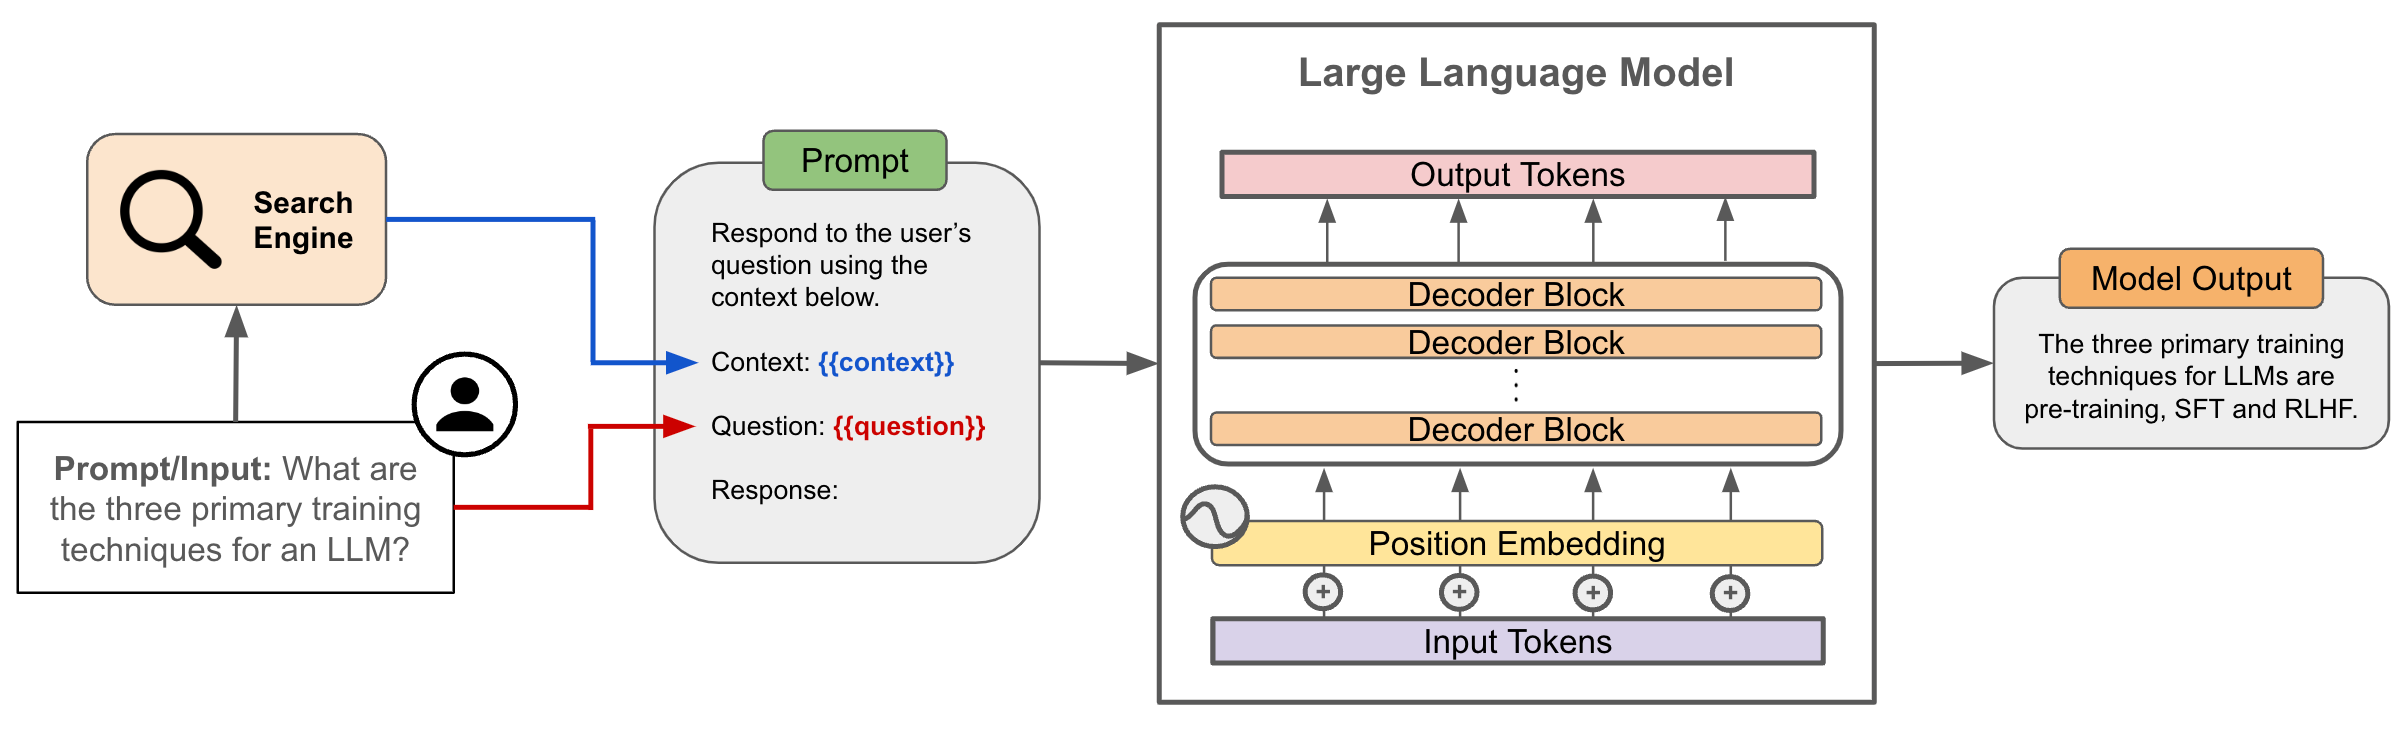
\includegraphics[width=0.9\textwidth]{img/pdz/13-generation.png}
    \caption{Generation \cite{wolfe2024_rag_guide}}
    \label{fig:Generation}
\end{figure}

Formally, given a query $q$ retrieves a document set $D = \{d_1, \dots, d_k\}$, the generator models the output sequence $y = (y_1, \dots, y_T)$ as:
\[
P(y \mid q, D) = \prod_{t=1}^{T} P(y_t \mid y_{<t}, q, D).
\]

Instead of treating retrieved documents as a single concatenated input, marginalization across documents can be applied:
\[
P(y_t \mid y_{<t}, q, D) = \sum_{d_i \in D} P(y_t \mid y_{<t}, q, d_i) \, P(d_i \mid q).
\]

Each retrieved document is encoded into a latent representation:
\[
h_i = f_{\text{enc}}(d_i),
\]
and decoding attends to these representations:
\[
P(y_t \mid y_{<t}, q, d_i) = \text{softmax}\!\left(W \cdot \text{Dec}(y_{<t}, h_i)\right).
\]

Modern RAG systems typically adopt large language models built upon autoregressive or encoder-decoder transformer architectures, with retrieved content integrated through concatenation, cross-attention, or late fusion mechanisms \cite{asai2023selfrag, yoon2024compact}. Cross-attention approaches encode retrieved contexts independently, allowing the decoder to selectively attend to relevant passages during token generation and improving evidence utilization at scale.

\begin{itemize}
    \item \textbf{Concatenation-based generation:} Retrieved passages are appended to the prompt; simple but limited by context length and prone to noisy retrieval.
    \item \textbf{Cross-attention generation:} Retrieved representations act as separate attention sources to improve semantic alignment and reduce positional bias \cite{he2024retrieval_coding}.
\end{itemize}

In cross-attention generation, retrieved representations form a secondary attention memory:
\[
\text{Attention}(Q, K_D, V_D) = \text{softmax}\left(\frac{QK_D^\top}{\sqrt{d_k}}\right)V_D,
\]
where $K_D, V_D$ are keys and values derived from retrieval encodings.

\begin{itemize}
    \item \textbf{Rerank-and-generate pipelines:} Only top-ranked chunks are passed to the generator after evidence filtration \cite{zhang2024llm_hallucination_code}.
    \item \textbf{Self-reflective iterative generation:} Retrieval, generation, and critique occur recursively to enhance factual accuracy and reasoning \cite{asai2023selfrag}.
\end{itemize}

To further improve faithfulness, contrastive losses can be incorporated to prefer evidence-grounded explanations:
\[
\mathcal{L}_{\text{faith}} = -\log \frac{\exp(s(y, D^+))}{\exp(s(y, D^+)) + \exp(s(y, D^-))},
\]
where $D^+$ contains supporting evidence and $D^-$ contains retrieved distractors. The score function $s(y, D)$ measures how well a generated output $y$ is grounded in a document set $D$, commonly implemented as a similarity function such as:
\[
s(y, D) = \cos\left(g(y), \, h(D)\right),
\]
where $g(y)$ encodes the generated text and $h(D)$ aggregates document embeddings (e.g., mean pooling or attention-weighted fusion).

\subsection{Prompt Engineering}

Prompt engineering refers to the design and optimization of input prompts used to condition and control the behavior of large language models (LLMs) during inference. Since prompts act as the primary interface between users and pretrained models, they provide a mechanism for steering responses without modifying model parameters \cite{brown2020language}.

A foundational line of work explores how different prompting formats affect task performance. \textbf{Zero-shot prompting} relies solely on natural language instructions, enabling the model to generalize based on pretrained knowledge without additional examples \cite{reynolds2021prompt}. \textbf{One-shot} and \textbf{few-shot prompting} extend this by including one or multiple demonstration pairs, allowing models to infer task structure through in-context examples rather than fine-tuning \cite{brown2020language}. This form of in-context learning has proven effective across classification, extraction, and reasoning tasks.
More advanced prompting strategies target reasoning quality. \textbf{Chain-of-Thought (CoT) prompting} encourages models to generate intermediate reasoning steps before producing a final answer, improving performance on multi-step logical and mathematical tasks \cite{wei2022cot}. Subsequent techniques such as self-consistency aggregate multiple sampled reasoning paths to enhance stability and accuracy \cite{wang2023selfconsistency}.

Prompt engineering also underpins efforts to produce \textbf{structured and reliable outputs}. Schema-based prompts can enforce formats such as JSON, bullet lists, and domain-specific templates, enabling seamless integration with downstream systems \cite{gpt4techreport}. These constraints reduce hallucinations and parsing failures in production settings. Modern APIs further extend this idea via function calling interfaces, where models output well-defined data structures rather than free-form text, improving determinism and safety in tool-augmented pipelines.
Early prompt engineering relied heavily on manual experimentation, making it labor-intensive and heuristic-driven. Recent research has shifted toward automated strategies that systematically search, optimize, or learn prompts using algorithmic techniques.
A direct approach to \textbf{automated prompt optimization} is searching over a space of candidate prompts and selecting the best-performing one based on validation metrics. This includes searching over instruction phrasing, ordering of few-shot examples, or choice of examples. Since exhaustive search is infeasible due to a large combinatorial space, recent work frames prompt selection as a multi-armed bandit or best-arm identification problem, where each prompt is an ``arm’’ with an unknown reward. For example, TRIPLE \cite{shi2024triple} uses bandit algorithms to balance exploration and exploitation under a limited query budget, yielding better prompts with fewer evaluations. Other approaches employ evolutionary search or Monte Carlo tree search, demonstrating that automated discovery can outperform manually engineered prompts.
Beyond discrete text search, another line of work treats prompts as continuous parameters. Prefix-Tuning \cite{li2021prefix} learns soft prompt vectors that steer model behavior without modifying model weights. AutoPrompt \cite{shin2020autoprompt} performs gradient-guided search over discrete tokens, iteratively updating trigger tokens based on gradient signals. AutoPrompt showed that masked language models can perform tasks such as sentiment classification and natural language inference near state-of-the-art accuracy without fine-tuning, and also demonstrated improved factual recall on probing benchmarks. These approaches bridge classic training with prompt design, though continuous prompts may sacrifice interpretability.
Other methods refine an initial human-written prompt through iterative edits. GrIPS \cite{prasad2023grips} applies gradient-free heuristic edits adding, removing, or reordering phrases and retains only modifications that improve performance, making it suitable for closed-source models. Notably, optimized prompts sometimes appear nonsensical to humans yet perform better, revealing model-specific quirks. Instruction Induction and Automatic Prompt Engineer (APE) \cite{zhou2022ape} generate candidate instructions using an LLM itself, then score and select the best. APE notably discovered a more effective variant of chain-of-thought prompting (``Let’s work this out in a step-by-step way to be sure we have the right answer.'') that exceeded human-designed prompts on tasks.
Recent work such as OPRO \cite{yao2023opro} frames prompt optimization as a task performed by the LLM itself. A meta-prompt maintains a history of candidate prompts and their performance, and the model proposes new candidates iteratively. This closes the optimization loop and enables the model to generate self-improving prompts. While promising, meta-prompting must avoid trivial variations and overfitting to validation data.
Reinforcement learning (RL) offers another avenue by treating prompts as actions optimized for a reward function, such as validation accuracy or human preference. RLPrompt \cite{deng2022rlprompt} applies policy gradients to optimize discrete prompt tokens, achieving improvements over manual baselines. Although less widely adopted due to large search spaces and sparse rewards, RL-based approaches align naturally with interactive and user-feedback-driven prompting scenarios.
These developments illustrate a shift from heuristic prompt crafting toward principled optimization pipelines, leveraging search, gradients, RL, and LLM-driven meta-optimization to discover high-performing prompts beyond human intuition.

Overall, prompt engineering has matured from ad-hoc phrasing tricks into a systematic methodology spanning demonstrations, reasoning scaffolds, structural constraints, and automated optimization. As LLMs scale and deploy into real-world applications, prompt engineering remains central to achieving reliable, controllable, and domain-aligned model behavior.

\newpage
